\section{Auswertung}
\label{sec:Auswertung}
Die Auswertung findet anhand der Versuchsanleitung '"Versuch Wärmepumpe"' statt\cite[S.14]{Anleitung-WP}
\subsection{Energiebilanz der Anlage und äußere Leistungszahl}
In diesem Teil werden die Leistungszahlen und die Energiebilanz der Anlage berechnet.

\subsubsection{Prüfung Heizleistung}
\label{subsubsec:Heizleistung}

Die Heizleistung oder auch Heizdurchfluss wird mit der \autoref{eq:110623_Heizleistung} berechnet:

\begin{equation}
\dot Q_{Kond}= \dot m \cdot cp_{W} \cdot (T_{V} - T_{R})
\label{eq:110623_Heizleistung}
\end{equation}

Im ersten Schritt wird der Massenstrom über den Volumenstrom nach \autoref{eq:230624_Massestrom_V_D} bestimmt werden.

\begin{equation}
    \dot{m}= \dot{V}\cdot \rho
    \label{eq:230624_Massestrom_V_D}
\end{equation}

Durch multiplizierens des gemessenen Volumenstroms mit der gegebenen Dichte von $\rho = 990 \frac{kg}{m^3}$ wird der Massenstrom bestimmt:
$$\dot{m}= 0,391 \cdot 10^{-3}\frac{m^3}{s} \cdot 990 \frac{kg}{m^3}=0,38 \frac{kg}{s}$$

Im zweiten Schritt wird die Heizleistung mithilfe des Massenstroms berechnet:

$$\dot Q_{Kond}= 0,38 \frac{kg}{s} \cdot 4,2 \frac{kJ}{kg \cdot K} \cdot (48 ^{\circ}C - 43 ^{\circ}C) = 8,14 \frac{kJ}{s}$$

Mit einem Massenstrom von 0,38 $\frac{kg}{s}$, einer Vorlauftemperatur von 48 °C und Rücklauftemperatur von 43 °C im Kondensator ergibt sich daraus mit Formel \ref{eq:110623_Heizleistung} eine Heizleistung von 8,14 $\frac{kJ}{s}$ bzw $kW$.
 Die gemessene Heizleistung beträgt von 8,3kW, was eine minimale Abweichung vom errechneten Wert darstellt.
\newpage
\subsubsection{Äußere Leistungszahl}
Die äußere Leistungszahl wird mit \autoref{eq:110623_aeußere Leistungszahl_tatsächlich} errechnet. 

\begin{equation}
\epsilon_{Real,Au"sen} = \frac{\dot Q_{Nutz}}{P_{el}}
\label{eq:110623_aeußere Leistungszahl_tatsächlich}
\end{equation}

Für $\dot Q_{Nutz}$ wird die Heizleistung des Kondensators von 8,14kW und für $P_{el}$ die gemessene Anlagenleistung von 2,3kW eingesetzt:

$$ \epsilon_{Real,Au"sen} = \frac{8,14 kW}{2,3 kW} = 3,54$$

Die ermittelte Leistungszahl beträgt 3,54.

\subsubsection{Wärmestrom im Verdampfer}
Um den aus der Umgebung aufgenommenen Wärmestrom zu bestimmen, muss die Gesamt-Energiebilanz der Anlage verwendet werden:

\begin{equation}
\dot Q_{Verd}=\dot Q_{Kond}-P_{el}
\label{eq:110623_aeußere Leistungszahl}
\end{equation}
Mit der berechneten Heizleistung von 8,14kW und einer elektrischen Leistung von 2304W unter verwendung von \autoref{eq:110623_aeußere Leistungszahl}
$$\dot Q_{Verd}= 8,14 kW-2,304 kW= 5,84kW $$


Der Verdampfer nimmt einen Wärmestrome von 5,84kW auf.
Der benötigte Luftvolumenstrom bei einer Abkühlung von 5K wird durch \autoref{eq:110623_benoetigter_Luftstrom} bestimmt:
\begin{equation}
\dot V_{L}=\frac{\dot Q_{Verd}}{\rho_{Luft} \cdot cp_{Luft} \cdot \Delta T}
\label{eq:110623_benoetigter_Luftstrom}
\end{equation}

Die gegebene Luftdichte  beträgt $\rho_L = 1,2\frac{kg}{m^3}$ und die Wärmekapazität $c_{pL}= 1\frac{kJ}{kg \cdot K}$. 
$$\dot V_{L}=\frac{5,84 kW}{ 1,2 \frac{kg}{m^3} \cdot 1 \frac{kJ}{kg \cdot K} \cdot 5K}= 0,973 \frac{m^3}{s}$$


Der benötigte Luftstrom beträgt nach Formel \ref{eq:110623_benoetigter_Luftstrom} 0,973$\frac{m^3}{s}$. 
\newpage
\subsubsection{Äußere Carnot-Leistungszahl der Anlage \texorpdfstring{$\epsilon_{Carnot,a}$}{}}
\label{subsubsec:Carnot}

Für die äußere Carnot-Leistungszahl der Anlage wird die Umgebungstemperatur $T_{U}=$ 24°C= 297,15K und die mittlere Temperatur der Nutzwärme benötigt.

\begin{equation}
T_{mN}= \frac{T_{Kessel}+T_{Rück}}{2}
\end{equation}
Die gemessenen Werte betragen für $T_{Kessel}=51,6^\circ$ und $T_{Rück}= 44,9^\circ$.
$$T_{mN}=\frac{51,6^{\circ}C+44,9^{\circ}C}{2}=48,25^{\circ}C= 321,4 K$$
Die mittlere Temperatur der Nutzwärme beträgt $321,4$K.

Die äußere Carnot-Leistungszahl berechnet sich dann wie folgt: 

\begin{equation}
\epsilon_{Carnot, Au"sen} = \frac{T_{mN}}{T_{mN}-T_{U}}
\label{eq:110623_aeußere Carnot Leistungszahl}
\end{equation}

$$\epsilon_{Carnot, Au"sen} = \frac{321,4 K}{321,4 K-297,15K} = 13,25$$

Sie beläuft sich dabei auf 13,25.
\newpage
\subsection{Arbeitsmittelkreislauf und innere Leistungszahlen}
\subsubsection{lg(p),h-Diagramm}
Entsprechend der Werte aus Messreihe 1, welche in \autoref{tab:Arbeitspunkte} zusammengefasst sind, kann das passende
lg(p)-h-Diagramm, mit den Arbeitspunkten 1-4 erstellt werden. Aus diesem Diagramm lassen sich die in \autoref{tab:Arbeitspunkte} ebenfalls
notierten Enthalpien ablesen.

\begin{table}[!h]
    \centering
    \caption{Arbeitspunkte entsprechend Messreihe 2}
    \label{tab:Arbeitspunkte}
    \begin{tabular}{|c|c|c|c|}
    \hline
        \rowcolor[HTML]{70AD47} 
        \multicolumn{1}{|l|}{\cellcolor[HTML]{70AD47}{\color[HTML]{000000} \textbf{Arbeitspunkt}}} & {\color[HTML]{000000} Bezeichnung} & \multicolumn{1}{l|}{\cellcolor[HTML]{70AD47}{\color[HTML]{000000} Temperatur in °C}} & \multicolumn{1}{l|}{\cellcolor[HTML]{70AD47}{\color[HTML]{000000} Enthalpie in kJ/kg}} \\ \hline
        \rowcolor[HTML]{CFE5A8} 
        1                                                                                          & Temperatur nach Verdampfer         & 18                                                                                   & 425                                                                                    \\ \hline
        \rowcolor[HTML]{E2EFDA} 
        2                                                                                          & Heißgastemperatur                  & 66                                                                                   & 453                                                                                    \\ \hline
        \rowcolor[HTML]{CFE5A8} 
        3                                                                                          & Verflüssigertemperatur             & 45                                                                                   & 276                                                                                    \\ \hline
        \rowcolor[HTML]{E2EFDA} 
        4                                                                                          & Temperatur vor Verdampfer          & 15                                                                                   & 276                                                                                    \\ \hline
    \end{tabular}
    \end{table}

    \begin{figure}[!h]
        \centering
        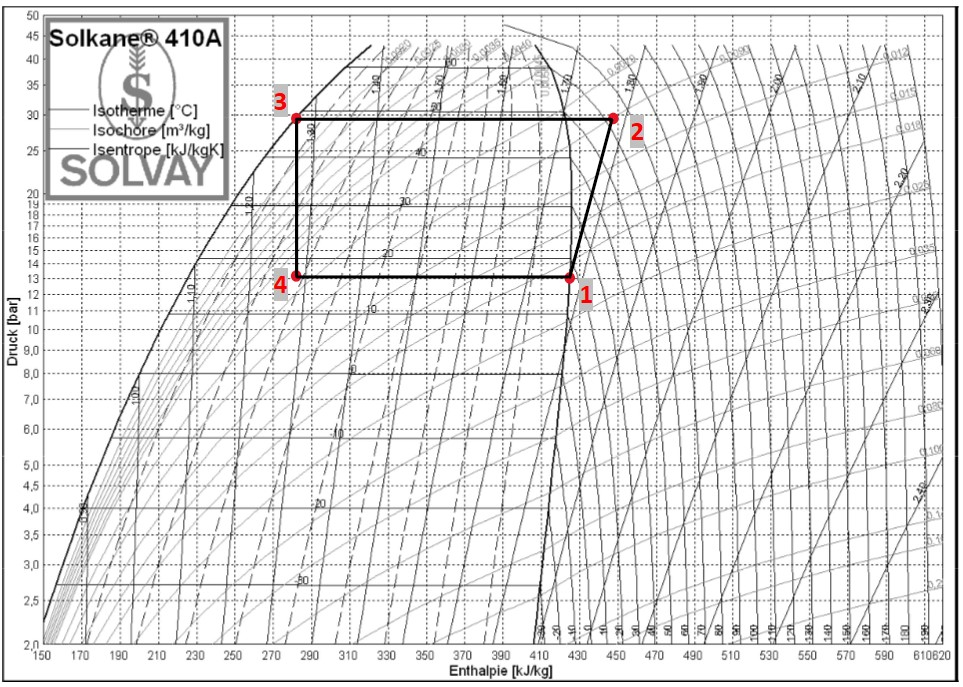
\includegraphics[width=\textwidth]{Abbildungen/lgp-h-diagramm.jpg}
        \caption{lg(p)-h-Diagramm für den realen Kreisprozess mit Darstellung der Irreversibilität}
        \label{fig:lgp-h-Diagramm}
    \end{figure}


    Zusätzlich kann das obere Druckniveau von 28 bar und das unter Druckniveau von rund 12,8 bar abgelesen werden.
    \autoref{fig:lgp-h-Diagramm} entspricht einem üblichen Kreisprozess, was die Plausiblität der Ergebnisse bestärkt. 
    Der minimale Anstieg der Temperatur von Punkt 4 zu Punkt 1 ist ungewöhnlich, allerdings durch einfache Fehler beim Messen oder Verluste am Verdampfer zu erklären.\\
\newpage
\subsubsection{Innere Carnot-Leistungszahl}
Mit den Temperaturen aus \autoref{tab:Arbeitspunkte} kann mittels \autoref{eq:Innere Carnot-Leistungszahl} die innere Carnot-Leistungszahl
ermittelt werden. 

    \begin{equation}
        \epsilon_{Carnot, Innen}=\frac{T_{max}}{T_{max}-T_{min}}=\frac{T_{Kond}}{T_{Kond}-T_{Verd}}
        \label{eq:Innere Carnot-Leistungszahl}
    \end{equation}

$$\epsilon_{Carnot, Innen}=\frac{318,15 K}{318,15 K-288,15 K}=10,605$$
Die Berechnung ergibt eine innere Carnot-Leistungszahl von 10,605.

\subsubsection{Isentropenwirkungsgrad}
 In \autoref{fig:lgp-h-Diagramm} ist zusätzlich der isentrope Arbeitspunkt 2 eingezeichnet und somit ist eine isentrope Enthalpie für diesen Arbeitspunkt von $445 \frac{kJ}{kg}$abzulesen.
Mittels der abgelesenen isentropen Enthalpie für Arbeitspunkt 2 wird mit \autoref{eq:Isentropenwirkungsgrad} der Isentropenwirkungsgrad ermittelt.
\begin{equation}
    \eta_{is}=\frac{h_{2,is}-h_{1}}{h_{2}-h_{1}}
    \label{eq:Isentropenwirkungsgrad}
\end{equation}

$$\eta_{is}=\frac{(445-425)\frac{kJ}{kg}}{(453-425)\frac{kJ}{kg}}=0,714$$

Der Isentropenwirkungsgrad für diesen Fall beträgt demnach 0,714.\\

\subsubsection{Innere Leistungszahlen}

Aus der Dampfdrucktafel für das Kältemittel R410a\cite{DDT-R410A} wurden die Werte $h"_{p0}=425,46 \frac{kJ}{kg}$ und $h_{pH}= 225,03 \frac{kJ}{kg}$ entnommen und mit den Werten aus \autoref{tab:Arbeitspunkte} in \autoref{eq:230623_Leistungszahl_VPI} eingesetzt

\begin{equation}
    \epsilon_{VP,i} = \frac{h_{2,is}-h_{pH}}{h_{2,is}-h^{''}_{p0}}
 \label{eq:230623_Leistungszahl_VPI}
 \end{equation}

 $$\epsilon_{VP,i}= \frac{(453-275,84)\frac{kJ}{kg}}{(453-425,46)\frac{kJ}{kg}} = 6,433 $$
 Die ermittelte innere Leistungszahl $\epsilon_{VP,i}$ beträgt 6,433.

 Die reale innere Leistungszahl wird durch \autoref{eq:230624_Leistungszahl_Reali} bestimmt:
 \begin{equation}
    \epsilon_{real,i}= \frac{h_2-h_3}{h_2-h_1}
    \label{eq:230624_Leistungszahl_Reali}
\end{equation}
Durch Einsetzen der Werte aus \autoref{tab:Arbeitspunkte} in \autoref{eq:230624_Leistungszahl_Reali}:
$$\epsilon_{real,i}= \frac{(453-276)\frac{kJ}{kg}}{(453-425)\frac{kJ}{kg}} = 6,321 $$
Die reale Leistungszahl beträgt 6,321.
\newpage
\subsection{Leistungszahlen und Verlustursachen}

\begin{table}[!ht]
    \centering
    \caption{Leistungszahlen in absteigender Reihenfolge}
    \label{tab:Leistungszahlen}
    \begin{tabular}{|l|l|l|}
        \hline
    \rowcolor[HTML]{70AD47} 
    {\color[HTML]{333333} \textbf{Leistungszahl}}  & {\color[HTML]{333333} \textbf{Wert}} & {\color[HTML]{333333} \textbf{Differenz}} \\
    \rowcolor[HTML]{C6E0B4} 
    $\epsilon_{Carnot,Au"sen}$ & 13,25                                & 0                                         \\ \hline
    \rowcolor[HTML]{E2EFDA} 
    $\epsilon_{Carnot,Innen}$  & 10,605                               & 2,645                                     \\ \hline
    \rowcolor[HTML]{C6E0B4} 
    $\epsilon_{VP,Innen}$      & 6,433                                & 4,172                                     \\ \hline
    \rowcolor[HTML]{E2EFDA} 
    $\epsilon_{Real,Innen}$    & 6,321                                & 0,112                                     \\ \hline
    \rowcolor[HTML]{C6E0B4} 
    $\epsilon_{Real,Au"sen}$   & 3,54                                 & 2,781                                     \\ \hline
    \end{tabular}%
    \end{table}

$\epsilon_{Carnot,Au"sen}$ gibt die maximale Leistungszahl an. 
Der äußere Carnot-Wirkungsgrad stellt einen idealisierten Prozess dar, bei dem Verluste vollständig vernachlässigt werden. 
Es werden lediglich die Temperaturänderung der mittleren Nutzwärme mit der Umgebungstemperatur verglichen.

Der äußere Carnot-Wirkungsgrad ist größer als der innere Carnot-Wirkungsgrad $\epsilon_{Carnot,Innen}$, da sich der innere auf die Kondensations- und Verdampfungstemperatur stützt. 
Um die Wärme auf den Prozess zu übertragen und wieder abzugeben, sind Temperaturunterschiede an den beiden Wärmetauschern erforderlich. 
Bei der Wärmepumpe erfolgt die Wärmeübertragung am Verdampfer und am Kondensator. 
Die Verluste der Wärmeübertragung werden beim inneren Carnot-Wirkungsgrad berücksichtigt.

Die innere Leistungszahl für den Vergleichsprozess $\epsilon_{VP,Innen}$ wurde mithilfe der theoretischen Enthalpien des Kältemittelkreislaufs berechnet.
Da die Werte aus Diagrammen oder auch Tabellen stammen können Abweichungen auftreten, da es eine Unschärfe bei der Übertragung der Messwerte auf Tabellendaten geben kann. 
Der theoretische Carnot-Prozess zur allgemeinen Wärmeübertragung wird durch einen realen Kältemittelkreislauf realisiert. 
Das Kältemittel Solkane 410A weist stoffspezifische Enthalpien auf. 
Es entstehen Verluste aufgrund des Stoffes und der tatsächlichen Prozessführung.

Die vorletzte Leistungszahl ist die reale innere Leistungszahl $\epsilon_{Real,Innen}$.
Der Wert ist geringer, da die Übergänge im realen nicht isentrop, sondern irreversibel verlaufen. 
Im Folgenden werden die Druck- und Reibungsverluste einzelner Bauteile berücksichtigt. 
Der Verdampfer sollte das Arbeitsmittel leicht überhitzen, da es sonst bereits in der Leitung zum Verdichter kondensieren könnte. 
Die Wärmezufuhr findet nicht wie theoretisch berechnet isobar statt.
Des Weiteren erfolgt die Verdichtung nicht isentrop und weist Verluste auf.

Im Kondensator ist das Arbeitsmittel überhitzt und gibt daher Wärme bei einer höheren Temperatur als der Kondensationstemperatur ab. 
Dadurch entstehen Wärme- und Druckverluste, ähnlich wie im Verdampfer. 
Die Kondensation findet aufgrund der Verluste ebenfalls nicht isobar statt
und auch die  Drossel arbeitet effizient, aber nicht vollständig isenthalp.
\\
Die geringste Leistungszahl ist die äußere Leistungszahl $\epsilon_{Real,Au"sen}$. 
Dieser Wert berücksichtigt den tatsächlich benötigten Nutzwärmestrom und die dafür erforderliche elektrische Verdichterleistung. 
Er umfasst daher alle Verluste im gesamten System.

\newpage
\subsection{Energiebilanzen Einzelapparate}
\label{subsec:Massenstrom}
\subsubsection{Arbeitsmittelmassenstrom Kondensator/Verdampfer}
Der Arbeitsmittelmassenstrom im Kondensator wird nach Formel \ref{eq:230623_massestrom} ermittelt.
\begin{equation}
   \dot m_{AM} = \frac{\dot Q_{Kond}}{|(h_3 - h_2)|}
   \label{eq:230623_massestrom}
\end{equation}

Mit $\dot Q_{Kondensator}=8,14kW$, $h_2=453\frac{kJ}{kg}$ und $h_3=276\frac{kJ}{kg}$ wird der Massenstrom des Kondensators nach \autoref*{eq:230623_massestrom} berechnet:

$$ \dot m_{AM_{Kond}} = \frac{8,14kW}{|(276\frac{kJ}{kg} - 453\frac{kJ}{kg})|} = 0,04746 \frac{kg}{s} $$
Der Massenstrom des Arbeitsmittels im Kondensator beträgt $0,04746 \frac{kg}{s}$.
\\
Analog erfolgt die Berechnung des Arbeitsmittelmassenstrom im Verdichter nach \autoref{eq230623_massestrom_ver}
\begin{equation}
  \dot m_{AM_{Verd}} = \frac{\dot Q_{Verd}}{|(h_1-h_4)|}
    \label{eq230623_massestrom_ver}
\end{equation}

Mit $\dot Q_{Verd}=5,84kW$, $h_1=425\frac{kJ}{kg}$ und $h_4=276\frac{kJ}{kg}$ wird der Massenstrom des Verdichters nach \autoref*{eq230623_massestrom_ver} berechnet:
$$\dot m_{AM} = \frac{5,84 kW}{|(425\frac{kJ}{kg}-276\frac{kJ}{kg})|} = 0,03907 \frac{kg}{s}$$
Der Massenstrom des Arbeitsmittels im Verdichter beträgt $0,03907 \frac{kg}{s}$.

$$\overline{\dot m}_{AM} = \frac{\dot m_{AM_{Kond}}+\dot m_{AM_{Verd}}}{2} = \frac{0,04746 \frac{kg}{s}+0,03907 \frac{kg}{s}}{2} = 0,04327 \frac{kg}{s} $$
Der Mittelwert des Arbeitsmittelmassenstroms beträgt $ 0,04327\frac{kg}{s}$.

\subsubsection{Verdichterleistung und Verdichterwirkungsgrad}

Die Verdichterleistung wird als mechanische Leistung nach \autoref{eq:230623_Verdichterleistung} berechnet.

\begin{equation}
    P_{mech} = \overline{\dot m}_{AM} \cdot (h_2-h_1)
\label{eq:230623_Verdichterleistung}
\end{equation}
Es wird der Mittelwert des Arbeitsmittelmassenstrom und die Enthalpiewerte aus Tabelle \ref{tab:Arbeitspunkte} eingesetzt:
$$  P_{mech} = 0,04327 \frac{kg}{s} \cdot (453-425)\frac{kJ}{kg} = 1,211 kW $$
Die mechanische Leistung beträgt 1211W.
\begin{equation}
  \eta_{Ver} = \frac{P_{mech}}{P_{el}}=\frac{\overline{\dot m}_{AM}\cdot (h_2-h_1)}{P_{el}}
\label{eq:230623_Verdichterwirkungsgrad}
\end{equation}
Für die Berechnung der Verdichterwirkungsgrad nach Formel \ref{eq:230623_Verdichterwirkungsgrad} wird die mechanische Leistung durch die elektrische Leistung geteilt.
$$\eta_{Ver} = \frac{1211W}{1800W}= 0,6728 \approx 67,28 \% $$
Der Wirkungsgrad des Verdichters beträgt 67,28 \%.
\subsubsection{Strömungsgeschwindigkeiten von Gas und Flüssigkeit}

Das spezifische Volumen des Gases kann aus dem lg(p)-h-Diagramm in \autoref{fig:lgp-h-Diagramm} abgelesen werden zu: $V_{Gas}=0,019 \frac{m^3}{kg}$. Die Dichte, welches der Kehrwert des spezifischen Volumens ist, ergibt sich als $\rho=52,63 \frac{kg}{m^3}$.
Der Durchmesser der Heißgasleitung beträgt 16 mm und der Kondensatleitung 10mm.
Mit dem durchschnittlichen Massenstrom aus \autoref{subsec:Massenstrom} können die Strömungsgeschwindigkeiten über den Volumenstrom nach folgenden Gleichungen berechnet werden.

\begin{equation}
    \dot{V}= \frac{\overline{\dot m}_{AM}}{\rho }
    \label{eq:230620_Volumenstrom}
\end{equation}

\begin{equation}
    \dot{V}= v \cdot \frac{\pi}{4} \cdot d^2
    \label{eq:230620_Volumenstrom2}
\end{equation}

Werden \autoref{eq:230620_Volumenstrom} und \autoref{eq:230620_Volumenstrom2} gleichgesetzt ergibt sich die Strömungsgeschwindigkeit nach \autoref{eq:230620_Strömungsgeschwindigkeiten}.

\begin{equation}
    v = \frac{\overline{\dot m}_{AM}}{\frac{\pi}{4}\cdot \rho \cdot d^2}
    \label{eq:230620_Strömungsgeschwindigkeiten}
\end{equation}
Am Arbeitspunkt 1 ergibt sich die Strömungsgeschwindigkeit:
$$v=\frac{0,04327 \frac{kg}{s}}{\frac{\pi}{4}\cdot 52,63 \frac{kg}{m^3} \cdot (0,016 m)^2}=4,089 \frac{m}{s} $$

Der Druck am Arbeitspunkt 3 kann aus dem lg(p)-h Diagramm als $p=28 bar$ abgelesen werden. Mithilfe dessen lässt sich die Dichte aus der Dampfdrucktafel als $\rho=935,99 kg/m^3$ bestimmen.
Die Strömungsgeschwindigkeit der Flüssigkeit am Arbeitspunkt 3 berechnet sich dann zu:
$$v=\frac{0,04327 \frac{kg}{s}}{\frac{\pi}{4}\cdot 935,99\frac{kg}{m^3} \cdot (0,01 m)^2}=0,588 \frac{m}{s}$$
\newpage
\subsubsection{T,A-Schaubild und K-Wert des Plattenwärmeübertragers}

\autoref{fig:TA,Diagramm} zeigt das T,A-Schaubild des kleinen Gegenstrom-Plattenwärmeübertragers
zwischen internem und externem Heizkreis.

\begin{figure}[!h]
    \centering
    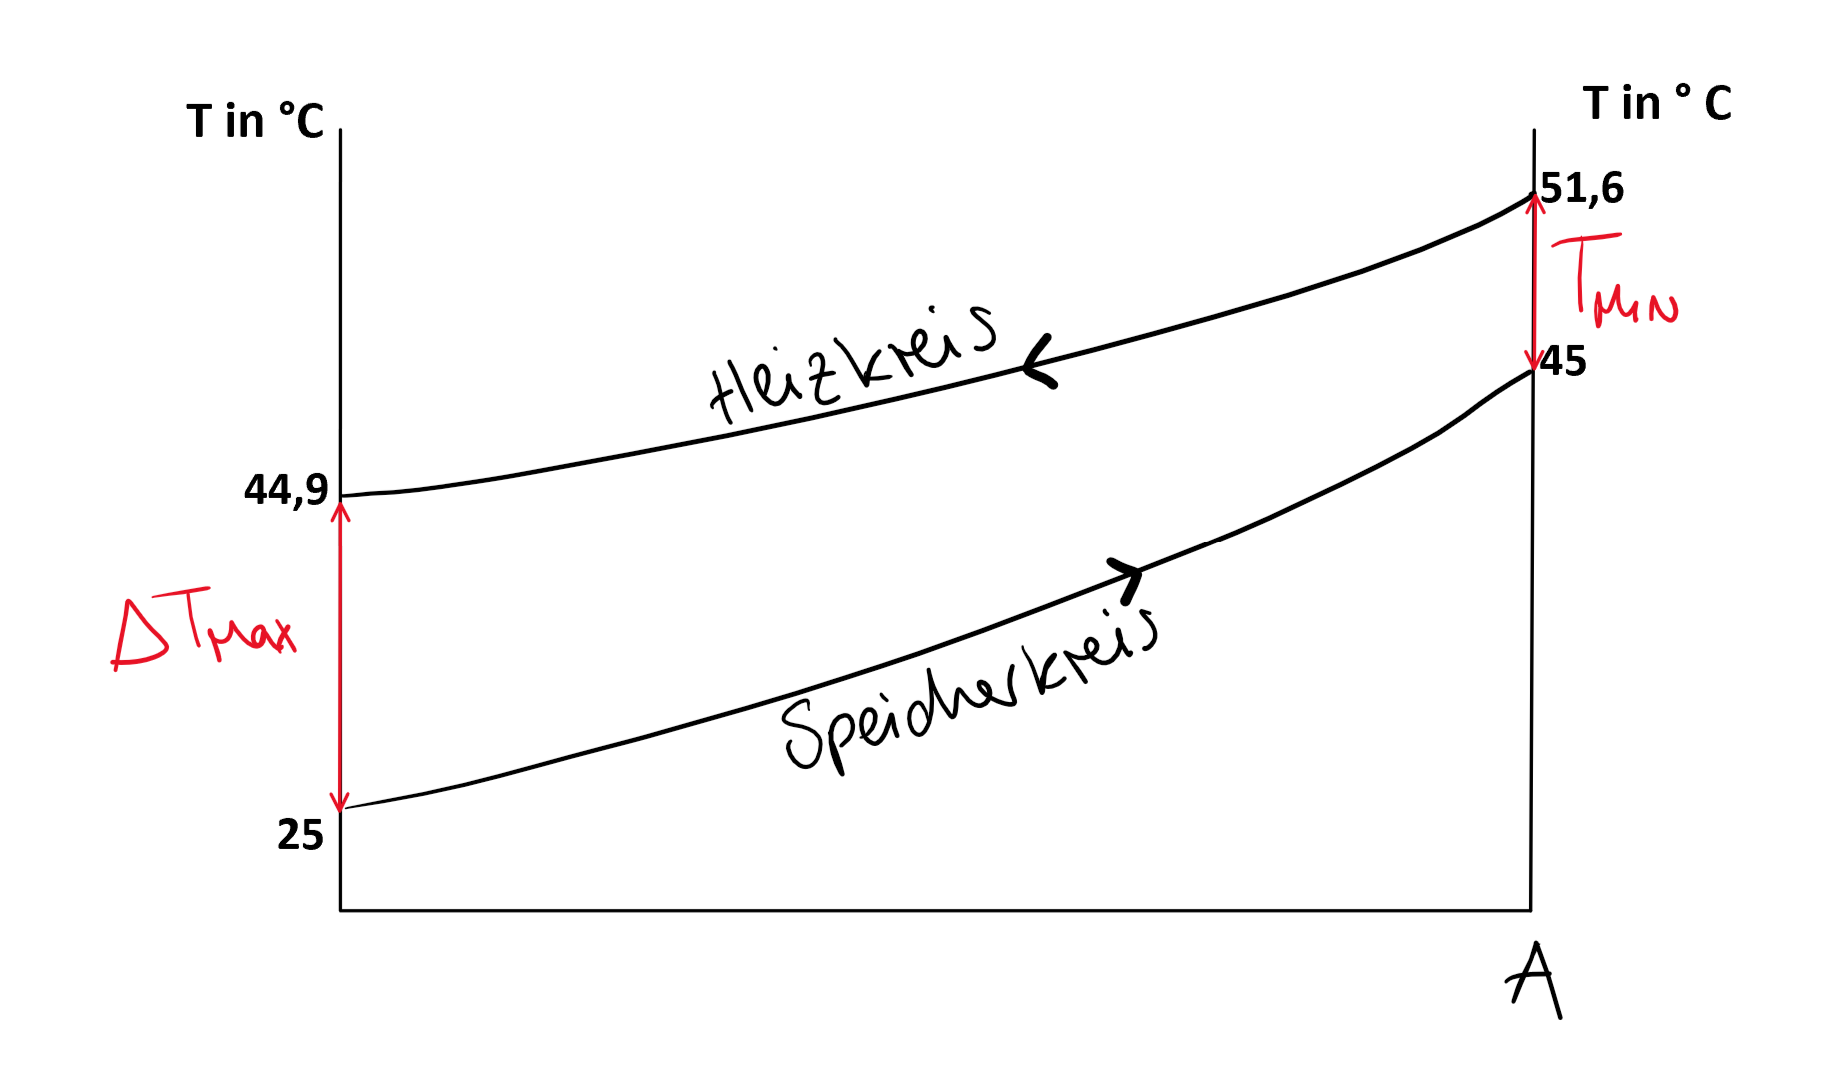
\includegraphics[width=0.6\textwidth]{Abbildungen/T_A_Diagramm.png}
    \caption{T,A-Schaubild eines Gegenstrom-Plattenwärmeübertragers}
    \label{fig:TA,Diagramm}
\end{figure}

\subsubsection*{K-Wert}
Für die Berechnung des K-Werts muss im Vorfeld $\Delta T_M$ bestimmt werden.
Im ersten Schritt wird die maximale Temperaturdifferenz wird aus der Speicher-Rücklauftemperatur und der Kesselrücklauftemperatur bestimmt.

\begin{equation}
    \Delta T_{MAX}= \Delta T_{HA}-\Delta T_{KE}
    \label{eq:230621_DeltaTMAX}
\end{equation}

$$\Delta T_{MAX}= 44,9\text{°}C-25 \text{°} C= 19,9K$$
Die maximale Temperaturdifferenz beträgt 19,9K.
Im zweiten Schritt wird die minimale Temperaturdifferenz aus der Speicher-Vorlauftemperatur und der tatsächlichen Kesseltemperatur berechnet.

\begin{equation}
    \Delta T_{MIN}= \Delta T_{HE}-\Delta T_{KA}
    \label{eq:230621_DeltaTMIN}
\end{equation}

$$\Delta T_{MIN}= 51,6 \text{°} C-45 \text{°} C= 6,6K$$
Die minimale Temperaturdifferenz beträgt 6,6K.\\
Im nächsten Schritt wird die mittlere Temperaturdifferenz bestimmt.
\begin{equation}
    \Delta T_{M}= \frac{\Delta T_{MAX}-\Delta T_{MIN}}{ln(\frac{\Delta T_{MAX}}{\Delta T_{MIN}})}
    \label{eq:230621_DeltaTM}
\end{equation}

$$\Delta T_M= \frac{19,9K-6,6K}{ln(\frac{19,9K}{6,6K})}= 12,05K$$
Die mittlere Temperaturdifferenz beträgt 12,05K.
\newpage
Mithilfe der \autoref{eq:230621_Q}, der gegebenen Fläche von $A= 0,4m^2$ und der Heizleistung lässt sich der k-Wert bestimmen, wobei Formel \ref*{eq:230621_Q} umgestellt nach k \autoref{eq:230621_k} ergibt.
\begin{equation}
    \dot{Q}=k\cdot A \cdot \Delta T_M
    \label{eq:230621_Q}
\end{equation}
\begin{equation}
    k = \frac{\dot{Q}}{ A \cdot \Delta T_M} 
    \label{eq:230621_k}
\end{equation}

$$k=\frac{8,14 kW}{ 0,4m^2 \cdot 12,05K}=1,69 \frac{kW}{m^2K}$$
Der ermittelte K-Wert beträgt 1,69 $\frac{kW}{m^2\cdot K}$.
\subsubsection{Aufheizen des gesamten Speichers}
Die Wärmemenge die benötigt wird um den Speicher aufzuheizen berechnet sich nach:
\begin{equation}
Q = m \cdot c_p \cdot \Delta T = \rho \cdot V \cdot c_p \cdot \Delta T
\label{eq230624_Qs}
\end{equation}
Durch das Umrechnen des Volumens von 450l mit der Dichte $\rho_W$ und einsetzen in Formel \ref{eq230624_Qs}:
$$ Q = 997 \frac{kg}{m^3} \cdot 0,45 m^3 \cdot 4,18 \frac{kJ}{kg K} (35 \text{°} C-21 \text{°} C)K=26,25 MJ$$
Die Wärmeenergie beträgt 26,25 MJ.
Die Heizleistung ist eine Energieangabe pro Zeiteinheit, wodurch die Zeit durch \autoref{eq:last} bestimmbar ist.

\begin{equation}
    P_{Heiz}= \frac{Q}{t}
    \label{eq:last}
\end{equation}

\begin{equation}
 t = \frac{Q}{P_{Heiz}}
\end{equation}

$$ t= \frac{26,25 MJ}{8,14 kW}=3224,82 s= 53,747 min$$
Um den gesamten Speicherinhalt aufzuheizen Bedarf es eines Betriebs von $\approx$ 54min.
\subsection{Zusatzaufgabe}

Die Exergie Verluste werden mithilfe des Carnot-Wirkungsgrads und der abgegebenen Nutzwärme bestimmt.
Der Carnot-Wirkungsgrad ist der Kehrwert der Carnot Leistungszahl, welche in \autoref{subsubsec:Carnot} als 13,25 berechnet ist.

\begin{equation}
    \eta_{Carnot}=\frac{1}{\epsilon_{Carnot}}=\frac{1}{13,25}= 7,5 \%
\end{equation}

Die Exergie Verluste ergeben dann:
\begin{equation}
   \Delta \dot{E}_V= \dot{Q}_{Nutz} \cdot\eta_{Carnot}
\end{equation}
$$\Delta \dot{E_V}= 8,14kW \cdot 7,5\%= 614W$$


\subsection{Fehlerbetrachtung}
Innerhalb der drei Messungen sinkt die Temperatur im Speicher,
trotz laufender Wärmepumpe. Ursächlich können verschiedene Faktoren sein. Der Speicher ist nicht mehr in die eigentliche Wärmedämmung gehüllt und wärmer als die Raumtemperatur. Der Abluftstrom ist in Richtung Speicher ausgerichtet. Da es eine erhöhte Konvektion gibt, könnte es zu einer beschleunigten Wärmeabgabe des Speichers kommen.
Ein weiterer Faktor könnte eine falsche Kalibrierung der Messgeräte sein oder Messfehler. Der Messfehler kann bei günstigeren Thermometern bis zu 2 Grad Celsius betragen.



